\documentclass[11pt]{article}

\usepackage{fullpage}
\usepackage{graphicx}
\usepackage{amsmath}
\usepackage{times,float}
%\usepackage{program}
\usepackage{subfigure}
%\usepackage{amsfonts}
%\usepackage{mathptm}

\textheight 48pc
\textwidth 38pc
\topmargin -3.0pc
\oddsidemargin 0pc
\evensidemargin -1pc
\marginparsep -1pc
\marginparwidth 0pc


\newcommand{\comment}[1]{\textit{\small {#1}}}
\newcommand{\cpp}{C\texttt{++}\ }
\newcommand{\tcl}{\textsc{Tcl\ }}
\newcommand{\ProtoMol}{\textsc{ProtoMol\ }}
\newcommand{\SamdII}{\textsc{Samd 2\ }}
\newcommand{\MOLLY}{\textsc{MOLLY\ }}

\newcommand{\tempstart}{\texttt{<}}
\newcommand{\tempend}{\texttt{>}}
\newcommand{\rij}{\mbox{r$_{ij}$}}
\newcommand{\rik}{\mbox{r$_{ik}$}}
\newcommand{\vrij}{\mbox{$\vec{r}_{ij}$}}
\newcommand{\Si}[1]{\mbox{Si$_{#1}$}}
\newcommand{\Vr}[1]{\mbox{$\vec{r}_{#1}$}}
\newcommand{\Vx}[1]{\mbox{$\vec{x}_{#1}$}}
\newcommand{\Vv}[1]{\mbox{$\vec{v}_{#1}$}}
\newcommand{\hatr}[1]{\mbox{$\hat{{r}_{#1}}$}}
\newcommand{\hatv}[1]{\mbox{$\hat{{v}_{#1}}$}}
\newcommand{\AbsVr}[1]{\mbox{$\left| \vec{r}_{#1} \right| $}}
\newcommand{\AbsVv}[1]{\mbox{$\left| \vec{v}_{#1} \right| $}}


\begin{document}
\title{
\begin{Large}
The Hessian of Angle Energy,
van de Waals Energy, \\ Electrostatic Energy 
and Switching Functions
\end{Large}
}
\author{Qun Ma \& Jes\'us Izaguirre}
\bigskip
\date{\today}
\maketitle

\parskip 0.3cm

%%%%%%%%%%%%%%%%%%%%%%%%%%%%%%%%%%%%%%%%%%%%%%%%%%%%%%%%%%%%%%%%%%%%%%%%%

\section{Mathematical Notations}
In this short paper we are going to show how the Hessian of a given
energy function is derived, in which some special mathematical notations 
are used. 
\begin{itemize}
\item Gradient. The gradient of a scalar variable $S$, w.r.t. a vector, 
$\vec{v} = (v_i, v_j, v_k)^T$ where $v_i$, $v_j$, $v_k$ are also
vectors, is defined as follows:
\begin{equation}
S_v \equiv \nabla_{\vec{v}} S \equiv \frac{\mathrm{d}S}
{\mathrm{d}\vec{v}} =
(\frac{\partial S}{\partial {v_i}},\frac{\partial S}{\partial v_j},
\frac{\partial S}{\partial v_k})^T. 
\end{equation}
\item Hessian. The Hessian is the gradient of the gradient of a scalar
variable $S$, w.r.t. a vector, 
$\vec{v} = (v_i, v_j, v_k)^T$ where $v_i$, $v_j$, $v_k$ are also
vectors, is defined as follows:
\begin{equation}
S_{vv} \equiv \nabla_{\vec{v}} S_v 
       \equiv \frac{\mathrm{d} S_v}{\mathrm{d} \vec{v}} =
\left[
\begin{tabular}{c c c}
$\frac{\partial^2 S}{\partial {v_i}^2}$ &
$\frac{\partial^2 S}{\partial {v_i} \partial {v_j}} $&
$\frac{\partial^2 S}{\partial {v_i} \partial {v_k}} $\\
$\frac{\partial^2 S}{\partial {v_j} \partial {v_i}} $&
$\frac{\partial^2 S}{\partial v_j^2} $&
$\frac{\partial^2 S}{\partial {v_j} \partial {v_k}} $\\
$\frac{\partial^2 S}{\partial {v_k} \partial {v_i}} $&
$\frac{\partial^2 S}{\partial {v_k} \partial {v_j}} $&
$\frac{\partial^2 S}{\partial v_k^2}$
\end{tabular}
\right]. 
\end{equation} 
\end{itemize}
For example, let $\left|\vec{v_{jk}}\right|$ be
the 2-norm of the vector $\vec{v_{jk}}$ where 
$v_{jk}= v_k - v_j$, and $\hat{v_{jk}}$ be the unit
vector with the direction of $\vec{v_{jk}},$ 
then the following statements are true where all the identity
matrices, $I$, have dimension of $3\times3:$
\begin{eqnarray}
\label{eg1}
\frac{\partial v_{jk}}{\partial{v_j}} &=& -I \\
\label{eg2}
\frac{\partial 
\left|\vec{v_{jk}}\right|}
{\partial{v_j}} &=& 
-\frac{\partial 
\left|\vec{v_{kj}}\right|}
{\partial{v_j}} =
 - \hat{v_{jk}} = \hat{v_{kj}}\\
\label{eg3}
\frac{\partial \hatv{kj}}
{\partial{v_j}} &=& \frac{\partial}{\partial{v_j}}
\left(  
\frac{\vec{v_{kj}}}{\AbsVv{kj}} \right) =  \frac{1}{\AbsVv{kj}}
(I - \hatv{kj}\hatv{kj}^T)\\
\label{eg4}
\frac{\partial 
\left|\vec{v_{jk}}\right|}
{\partial{v}} &=& [0,\,-1,1]^T \, \hat{v_{jk}}
\end{eqnarray}
where $\hatv{jk} = \frac{\Vv{jk}}{\AbsVv{jk}}$ is the unit vector in
the direction of $\Vv{jk},$ $\hatv{kj}\hatv{kj}^T$ is the outerproduct 
of $\hatv{kj}$ and $\hatv{kj}$ as defined in the following equation,
assumming $v_k = [x_k, y_k, z_k]^T$ and $v_j = [x_j,y_j, z_j]^T:$
\begin{equation}
\hatv{kj}\hatv{kj}^T
= \frac{1}{\AbsVv{kj}^2}\left[ \begin{array}{ccc}
x_{kj} x_{kj}  & x_{kj} y_{kj}  & x_{kj} z_{kj} \\
y_{kj} x_{kj}  & y_{kj} y_{kj}  & y_{kj} z_{kj} \\
z_{kj} x_{kj}  & z_{kj} y_{kj}  & z_{kj} z_{kj} 
\end{array}
\right].
\end{equation}
If we let $F = (0, v_{jk}, -v_{jk})^T,$ the following equation is also true:
\begin{equation}
\label{eg5}
\frac{\mathrm{d} F}{\mathrm{d}\vec{v}}
= \left[ \begin{array}{ccc}
0 & 0 & 0\\
0 & -I & I\\
0 & I & -I
\end{array}
\right].
\end{equation}

When expanded, the above equations are consistent with the regular
mathematical notations, {\it i.e.}, the Cartesian coordinates
expressed as $(x, y, z)$. In Equation~({\ref{eg1}}), the l.h.s refers
to the Hessian matrix. If $v_k = [x_k, y_k, z_k]^T$ and $v_j = [x_j,
y_j, z_j]^T$, then
\begin{equation}
\frac{\partial v_{jk}} {\partial{v_j}} = 
\left[ \begin{array}{ccc}
\frac{\partial (x_k - x_j)} {\partial x_j} & 
\frac{\partial (x_k - x_j)} {\partial y_j} &
\frac{\partial (x_k - x_j)} {\partial z_j} \\
\frac{\partial (y_k - y_j)} {\partial x_j} & 
\frac{\partial (y_k - y_j)} {\partial y_j} &
\frac{\partial (y_k - y_j)} {\partial z_j} \\
\frac{\partial (z_k - z_j)} {\partial x_j} & 
\frac{\partial (z_k - z_j)} {\partial y_j} &
\frac{\partial (z_k - z_j)} {\partial z_j} 
\end{array}
\right] = - I. \\
\end{equation}
In Equation~(\ref{eg2}), the l.h.s refers to a vector:
\begin{equation}
\frac{\partial \AbsVv{jk}} {\partial{v_j}} = 
\left[ \begin{array}{r}
\frac{\partial \AbsVv{jk}}{\partial x_j} \\
\frac{\partial \AbsVv{jk}}{\partial y_j}\\
\frac{\partial \AbsVv{jk}}{\partial z_j}
\end{array}
\right] = 
- \left[ \begin{array}{r}
x_k-x_j \\
y_k-y_j \\
z_k-z_j  
\end{array}
\right]
\frac{1}{\AbsVv{jk}} = - \hatv{jk}
\end{equation}
where $\AbsVv{jk} = \sqrt{(x_k-x_j)^2+(y_k-y_j)^2+(z_k-z_j)^2}.$
In equation~({\ref{eg3}}), we want to get the Hessian of a unit
vector. Let $H_{kjj} = \frac{\partial \hatv{kj}}{\partial{v_j}},$ then

\begin{eqnarray}
H_{kjj} (1,1) &=& \frac{\partial }{\partial{x_j}}
\left(\frac{x_j - x_k}{\AbsVv{kj}} \right) =
\frac{1}{\AbsVv{kj}} - \frac{(x_j-x_k)^2}{\AbsVv{kj}^3}\\
H_{kjj} (1,2) &=& \frac{\partial }{\partial{y_j}}
\left(\frac{x_j - x_k}{\AbsVv{kj}} \right) =
-\frac{(x_j-x_k) (y_j-y_k)}{\AbsVv{kj}^3}\\
H_{kjj} (1,3) &=& \frac{\partial }{\partial{z_j}}
\left(\frac{x_j - x_k}{\AbsVv{kj}} \right) =
- \frac{(x_j-x_k) (z_j-z_k)}{\AbsVv{kj}^3}\\
H_{kjj} (2,1) &=& \frac{\partial }{\partial{x_j}}
\left(\frac{y_j - y_k}{\AbsVv{kj}} \right) =
- \frac{(x_j-x_k) (y_j-y_k)}{\AbsVv{kj}^3}\\
H_{kjj} (2,2) &=& \frac{\partial }{\partial{y_j}}
\left(\frac{y_j - y_k}{\AbsVv{kj}} \right) =
\frac{1}{\AbsVv{kj}} - \frac{(y_j-y_k)^2}{\AbsVv{kj}^3}\\
H_{kjj} (2,3) &=& \frac{\partial }{\partial{z_j}}
\left(\frac{y_j - y_k}{\AbsVv{kj}} \right) =
- \frac{(y_j-y_k) (z_j - z_k)}{\AbsVv{kj}^3}\\
H_{kjj} (3,1) &=& \frac{\partial }{\partial{x_j}}
\left(\frac{z_j - z_k}{\AbsVv{kj}} \right) =
-\frac{(x_j-x_k) (z_j - z_k)}{\AbsVv{kj}^3}\\
H_{kjj} (3,2) &=& \frac{\partial }{\partial{y_j}}
\left(\frac{z_j - z_k}{\AbsVv{kj}} \right) =
-\frac{(y_j-y_k) (z_j-z_k)}{\AbsVv{kj}^3}\\
H_{kjj} (3,3) &=& \frac{\partial }{\partial{z_j}}
\left(\frac{z_j - z_k}{\AbsVv{kj}} \right) =
\frac{1}{\AbsVv{kj}} - \frac{(z_j-z_k)^2}{\AbsVv{kj}^3}.
\end{eqnarray}
It is seen that $H_{kjj} = \frac{1}{\AbsVv{kj}} (I -
\hatv{kj}\hatv{kj}^T),$ thus Equation (\ref{eg3}) is verified.

Equation~({\ref{eg4}}) can be thought of a vector of vectors. When
using $(x_i,y_i,z_i,x_j,y_j,z_j,x_k,y_k,z_k)$ as the independent
variables instead of $(r_i, r_j, r_k)$, the vector is
\begin{equation}
\frac{\partial 
\left|\vec{v_{jk}}\right|}
{\partial{v}} = \frac{1}{\AbsVv{jk}}
 [0,0,0,-x_{jk},-y_{jk},-z_{jk},x_{jk},y_{jk},z_{jk}]^T
\end{equation}
which is consistent with Equation~({\ref{eg4}}).



\section{The Hessian of Angle Energy}
The Hessian matrices of the angle energy, van der Waals energy, and
electrostatic energy are useful in the mollification process 
in MOLLY integrators. The derivation of these formulae becomes
straightforward when the above mathematical notations are
used. Otherwise, it is forbiddenly burdensome, even if doable, to
derive them directly using the formal mathematical notations and the
cartesian coordinates $(x, y, z)$. This is specially true for the case 
of deriving Hessian of angle energy.

\subsection{Angle Energy and Force}
Angle interactions describe angular bonds between three atoms. These bonds are
modeled as harmonic angular springs. The layout of three such atoms
are illustrated as in Figure~\ref{3atoms} in which the heavy lines
indicate atoms $i$ and $j$, $j$ and $k$ are ``connected'' by the linear bonds
between them, and the dashed line indicates that there does not exist
linear bonds between atoms $i$ and $k$.
\begin{figure}[hbt]
\centerline{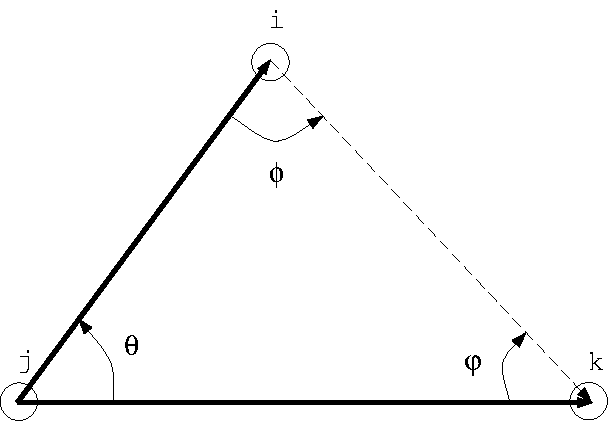
\includegraphics[width=1.5in]{3atoms.pdf}}
\caption{Layout of 3 atoms}
\label{3atoms}
\end{figure}

The energy of such a bond between atoms $i$, $j$,  and $k$ is given by:
\begin{eqnarray}
  E_{angle}  & = & E_{\theta} + E_{\mathrm{ub}} \label{eq:AngleEnergy} \\
  E_{\theta} & = & k_{\theta} \left( \theta - \theta_0 \right)^2   \\
\label{Eub}
  E_{\mathrm{ub}}     & = & k_{\mathrm{ub}} \left( \AbsVr{ik} - r_{\mathrm{ub}} \right)^2
\end{eqnarray}
\noindent
\\
where\\
\begin{tabular}{lcl}
 $ k_{\theta} $ & =  & Force constant specified in the parameter file for this bond type.\\
 $\theta $ & = &  $\cos^{-1} \left( \frac{ \Vr{ij}\, \cdot \,\Vr{kj}
}{ \AbsVr{ij} \AbsVr{kj} } \right),$ which is equivalent to
$\tan^{-1}(\mbox{$\left| {\Vr{ij} \times \Vr{kj}} \right|$}, \Vr{ij} \cdot \Vr{kj})$ \\
$ \theta_0 $   & = & Rest angle of this bond specified in the parameter file for this angle type.\\
$k_{\mathrm{ub}}$ &=& Urey-Bradley constant, which defaults to zero \\
  \Vr{ik}       & = & \Vr{k} - \Vr{i} \\
  \AbsVr{ik}    & = &  $ \sqrt{(x_k - x_i)^2 + (y_k - y_i)^2 + (z_k - z_i)^2},$
                calculated distance between atoms $i$ and $k$.\\
  $ r_{\mathrm{ub}} $    & = & Rest distance for the Urey-Bradley term.
\end{tabular}


By differentiating this formula, the force for this bond can be found to be:
\begin{equation}
\vec{F}_{angle} = - \frac{\mathrm{d} E_{\mathrm{angle}}}{\mathrm{d} \vec{r}} \label{eq:angleForce}
                = \vec{F}_{\theta} + \vec{F}_{\mathrm{ub}}
\end{equation}
where
\begin{eqnarray*}
\vec{F}_{\theta} = - \frac{\mathrm{d} E_{\theta}}
	{\mathrm{d} \theta} \,\frac{\mathrm{d} \theta}{\mathrm{d} \vec{r} }
                = - 2k_{\theta}(\theta - \theta_0) \,\frac{\mathrm{d}
	 \theta}{\mathrm{d} \vec{r} }\\
\vec{F}_{\mathrm{ub}} = - \frac{\mathrm{d} E_{\mathrm{ub}}}
	{\mathrm{d} \vec{r}} = 2 k_{\mathrm{ub}} \left(
\AbsVr{ik} - r_{\mathrm{ub}} \right) \hatr{ik}
\end{eqnarray*}
where $\hatr{ik}$ is the unit vector in the direction of $\vec{r_{ik}}.$

Hence the angle force on atoms $i$, $j$, and $k$ is calculated as:
\begin{eqnarray}
\label{force_i}
   F_{\vec{r}}^i & = & 
             \frac{ 2k_{\theta}(\theta - \theta_0) }{
\sin(\theta) \AbsVr{ij} } 
             \left( \frac{ \vec{r_{ij}} \, \cos(\theta) }{ \AbsVr{ij}
} - \frac{\vec{r_{kj}}}{\AbsVr{kj} } \right) 
             + 2 k_{\mathrm{ub}} \left( \AbsVr{ik} - r_{\mathrm{ub}} \right)
\frac{\vec{r_{ik}}}{\AbsVr{ik}}\\
\label{force_k}
   F_{\vec{r}}^k & = & 
            \frac{ 2k_{\theta}(\theta - \theta_0) }{
\sin(\theta) \AbsVr{kj} } 
             \left( \frac{ \vec{r_{kj}} \, \cos(\theta) }{ \AbsVr{kj}
} - \frac{\vec{r_{ij}}}{\AbsVr{ij} } \right) 
             + 2 k_{\mathrm{ub}} \left( \AbsVr{ik} - r_{\mathrm{ub}} \right)
\frac{\vec{r_{ki}}}{\AbsVr{ik}} \\
\label{force_j}
   F_{\vec{r}}^j & = & - ( F_{\vec{r}}^i + F_{\vec{r}}^k ).
\end{eqnarray}

\subsection{The Proof of the Force Expression}
The proof of the force expression follows a straight-forward approach
-- application of ``chain rule.'' Let 
\begin{equation}
C(\alpha, \beta, \gamma)=\frac{\alpha + \beta - \gamma}{2
\sqrt{\alpha}\sqrt{\beta}} 
\end{equation}
where $\alpha$, $\beta$ and $\gamma$ are scalars, 
\begin{eqnarray}
\alpha &=&\AbsVr{ij}^2 \\
\beta &=& \AbsVr{kj}^2 \\
\gamma &=& \AbsVr{ki}^2.
\end{eqnarray}
It then follows that the angle energy can be expressed as 
\begin{equation}
E_{\theta}(C(\alpha, \beta, \gamma)) = k_{\theta} (\theta - \theta_{0})^2
\end{equation}
where
$\theta = \cos^{-1}(C(\alpha, \beta, \gamma))$ since $\frac{ \Vr{ij}\,
\cdot \,\Vr{kj}}{ \AbsVr{ij} \AbsVr{kj}} = C(\alpha, \beta, \gamma). $
The force (negative gradient of the energy) is derived as follows:
\begin{equation}
F_{\theta} = - 
\nabla_{\vec{r}}E_{\theta} \equiv - E_r = - E_{C} \,C_r
\end{equation}
where 
$\vec{r} = (\Vr{i},\Vr{j},\Vr{k})$, and
\begin{eqnarray}
E_{C}&\equiv& \frac{\mathrm{d}E_{\theta}}{\mathrm{d}C} 
=  - \frac{2 k_{\theta} (\theta - \theta_0)}{\sqrt{1-C^2}} 
=  - \frac{2 k_{\theta} (\theta - \theta_0)}{\sin\theta}, \\
C_r  &\equiv& 
\nabla_{\vec{r}} C = f \, \alpha_r + 
g \, \beta_r + 
h \, \gamma_r,
\end{eqnarray}
where
\begin{eqnarray}
f &\equiv& \frac{\partial C}{\partial \alpha} =
\frac{\alpha - \beta + \gamma} 
{4\,\alpha^{3/2}\sqrt{\beta}} \\
g &\equiv& \frac{\partial C}{\partial \beta} = 
\frac{-\alpha + \beta + \gamma}
{4\,\sqrt{\alpha}\, \beta^{3/2}} \\
h &\equiv& \frac{\partial C}{\partial \gamma} 
= -\frac{1}{2\, \sqrt{\alpha}\, \sqrt{\beta}} \\
\alpha_{r} &\equiv&  \frac{\mathrm{d}\alpha}{\mathrm{d}\vec{r}} = (-2, 2, 0)^T
\sqrt{\alpha} \,\,\hatr{ij} \\
 \beta_{r} &\equiv& \frac{\mathrm{d}\beta}{\mathrm{d}\vec{r}} = (0, 2, -2)^T 
\sqrt{\beta} \,\,\hatr{kj}\\
\gamma_{r} &\equiv& \frac{\mathrm{d}\gamma}{\mathrm{d}\vec{r}} = (2, 0, -2)^T 
\sqrt{\gamma} \,\,\hatr{ki}.
\end{eqnarray}

It follows that the force acted on atom $i$ is expressed as
\begin{equation}
F_{\theta}^{i} = - E_C\,(-2 \sqrt{\alpha} \hatr{ij} \, f +
2 \sqrt{\gamma} \hatr{ki} \, h).
\end{equation}
Because $\sqrt{\gamma} \, \hatr{ki} = \vec{r_{kj}}\,- \, \vec{r_{ij}}$ 
and $\sqrt{\alpha} \, \hatr{ij} = \vec{r_{ij}},$
one has
\begin{eqnarray}
F_{\theta}^{i} &=& \frac{2 k_{\theta} (\theta - \theta_0)}{\sin\theta}\,
(-2 \vec{r_{ij}} \, f +
2 (\vec{r_{kj}}\,- \, \vec{r_{ij}}) \, h)\nonumber \\
&=& \frac{2 k_{\theta} (\theta - \theta_0)}{\sin\theta}\,
(-2 \vec{r_{ij}}\, \frac{\alpha - \beta + \gamma} 
{4\,\alpha^{3/2}\sqrt{\beta}} +
(\vec{r_{kj}}\,- \, \vec{r_{ij}}) (-\frac{1}{\sqrt{\alpha}\,
\sqrt{\beta}})) \nonumber \\
&=& \frac{2 k_{\theta} (\theta - \theta_0)}{\sin\theta}\,
(- \frac{\alpha - \beta + \gamma} 
{2\,\alpha^{3/2}\sqrt{\beta}}\,\vec{r_{ij}} +
\frac{1}{\sqrt{\alpha}\,
\sqrt{\beta}}  \vec{r_{ij}} \,-\,\frac{1}{\sqrt{\alpha}\,
\sqrt{\beta}}  \vec{r_{kj}})\nonumber \\
&=& \frac{2 k_{\theta} (\theta - \theta_0)}{\sin\theta}\,
(\frac{\alpha + \beta - \gamma} 
{2\,\alpha^{3/2}\sqrt{\beta}}\,\vec{r_{ij}} \,-\,\frac{1}{\sqrt{\alpha}\,
\sqrt{\beta}}  \vec{r_{kj}})\nonumber \\
&=& \frac{2 k_{\theta} (\theta - \theta_0)}{\sin\theta}\,
(\frac{1}{\alpha} \frac{\alpha + \beta - \gamma} 
{2\,\sqrt{\alpha} \sqrt{\beta}}\,\vec{r_{ij}} \,-\,\frac{1}{\sqrt{\alpha}\,
\sqrt{\beta}}  \vec{r_{kj}})\nonumber \\
& = & \frac{ 2k_{\theta}(\theta - \theta_0) }{ \sin(\theta) \AbsVr{ij}
} \left( \frac{ \vec{r_{ij}} \, \cos(\theta) }{ \AbsVr{ij} } -
\frac{\vec{r_{kj}}}{\AbsVr{kj} } \right).
\end{eqnarray}

The Urey-Bradley force acted on atom $i$ is as follows:
\begin{equation}
\vec{F}_{\mathrm{ub}}^i = 2 k_{\mathrm{ub}} (
\AbsVr{ik} - r_{\mathrm{ub}} ) \frac{\vec{r_{ik}}}{\AbsVr{ik}}
\end{equation}

The total force is the sum of the two terms. It is seen that the
force on atom $i$ is same as given in Equation~({\ref{force_i}}). One
can use the symetry of atoms $i$ and $k$ to verify the correctness of 
Equation~({\ref{force_k}}). The correctness of Equation~({\ref{force_j}})
can be verified using the second law of force by Newton, ``The force
acted on object $i$ by object $j$ is same as that acted on object $j$ by
object $i$ in magnitude but in the opposite direction.'' End of proof.

\subsection{The Hessian of Angle Energy}
By definition, the Hessian is the second
derivative of the energy function, or the first derivative 
of the gradient of energy. The Hessian of the Urey-Bradley energy as
shown in Equation~(\ref{Eub}) can be obtained easily.

\begin{eqnarray}
  E^{\mathrm{ub}}_r  &\equiv& \nabla_{\vec{r}}E_{\mathrm{ub}} =  2 k_{\mathrm{ub}} \left(
\AbsVr{ik} - r_{\mathrm{ub}} \right) [-\hatr{ik}, 0, \hatr{ik}]^T \\
  E^{\mathrm{ub}}_{rr}  &\equiv& \nabla_{\vec{r}}E^{\mathrm{ub}}_r 
= 2 k_{\mathrm{ub}} \frac{\AbsVr{ik} - r_{\mathrm{ub}}}{\AbsVr{ik}}
\left[ \begin{array}{ccc}
I & 0 & -I\\
0 & 0 & 0\\
-I & 0& I
\end{array}
\right] \nonumber \\ 
& & + \frac{2 \,k_{\mathrm{ub}}\, r_{\mathrm{ub}}}{\AbsVr{ik}}
\left[ \begin{array}{ccc}
\hatr{ik}\hatr{ik}^T & 0 & -\hatr{ik}\hatr{ik}^T\\
0 & 0 & 0\\ 
-\hatv{ik}\hatv{ik}^T & 0& \hatr{ik}\hatr{ik}^T
\end{array}
\right].
\end{eqnarray}

Now let's show the second derivative of the $E_\theta$ part. 
\begin{equation}
\label{Err}
\frac{\mathrm{d} E_r}{\mathrm{d} r} \equiv E_{rr} = \overbrace{E_{C} \,C_{rr}}^{E_{rr}^a}
+ \underbrace{C_{r} \,\, E_{Cr}^T}_{E_{rr}^b}
\end{equation}
where
\begin{equation}
E_{Cr} \equiv \nabla_{\vec{r}} \, E_{C}  
= E_{CC}\,C_{r},
\end{equation}
and
\begin{equation}
E_{CC} \equiv \frac{\mathrm{d} E_{C}}{\mathrm{d} C}
= \frac{2\,k_{\theta}[\sin\theta - 
(\theta - \theta_0)\cos\theta]}{\sin^3\theta},
\end{equation}
and
\begin{equation}
C_{rr} \equiv \nabla_{\vec{r}}C_{r} = 
\overbrace{
(f \, \alpha_{rr} + 
g \, \beta_{rr} + 
h \, \gamma_{rr})
}^{C_{rr}^a}
 + 
\underbrace{
(\alpha_{r} \, f_r^T + 
\beta_{r} \, g_r^T + 
\gamma_{r} \, h_r^T)
}_{C_{rr}^b},
\label{Crr1}
\end{equation}
where
\begin{eqnarray}
\alpha_{rr} &\equiv& \frac{\mathrm{d} \alpha_r}{\mathrm{d} \vec{r}} 
= \left[ \begin{array}{ccc}
2 I& -2 I & 0\\
-2 I& 2 I& 0\\
0 & 0& 0
\end{array}
\right]\\
\beta_{rr} &\equiv& \frac{\mathrm{d} \beta_r}{\mathrm{d} \vec{r}} 
= \left[ \begin{array}{ccc}
0 & 0& 0 \\
0 & 2 I & -2 I\\
0 & -2 I& 2 I
\end{array}
\right]\\
\gamma_{rr} &\equiv& \frac{\mathrm{d} \gamma_r}{\mathrm{d} \vec{r}} 
= \left[ \begin{array}{ccc}
2 I& 0 &-2 I \\
0 & 0& 0 \\
-2 I& 0 &2 I
\end{array}
\right]
\end{eqnarray}
and
\begin{eqnarray}
f_r &\equiv& \frac{\mathrm{d}}{\mathrm{d} r}f(\alpha, \beta, \gamma)
=f_\alpha \, \alpha_r + 
f_\beta \, \beta_r + 
f_\gamma \, \gamma_r \\
g_r &\equiv& \frac{\mathrm{d}}{\mathrm{d} r}g(\alpha, \beta, \gamma)
=g_\alpha \, \alpha_r + 
g_\beta \, \beta_r + 
g_\gamma \, \gamma_r \\
h_r &\equiv& \frac{\mathrm{d}}{\mathrm{d} r}h(\alpha, \beta, \gamma)
=h_\alpha \, \alpha_r + 
h_\beta \, \beta_r + 
h_\gamma \, \gamma_r \\
\end{eqnarray}
where
\begin{eqnarray}
f_\alpha &\equiv& \frac{\partial f}{\partial \alpha} =
\frac{-\alpha + 3\beta - 3\gamma} 
{8 \,\alpha^{5/2}\,\sqrt{\beta}} \\
f_\beta &\equiv& \frac{\partial f}{\partial \beta} =
\frac{-\alpha - \beta - \gamma}
{8 \,\alpha^{3/2}\,\beta^{3/2}}\\
f_\gamma &\equiv&\frac{\partial f}{\partial \gamma} =
\frac{1}{4 \alpha^{3/2}\, \sqrt{\beta}} \\
g_\beta &\equiv& \frac{\partial g}{\partial \beta} = 
\frac{3\alpha - \beta - 3\gamma}
{8 \,\sqrt{\alpha}\,\beta^{5/2}} \\
g_\gamma &\equiv& \frac{\partial g}{\partial \gamma} =
\frac{1}{4 \,\sqrt{\alpha}\, \beta^{3/2}} \\
h_\gamma &\equiv&\frac{\partial h}{\partial \gamma} = 0 \\
g_\alpha &\equiv& \frac{\partial g}{\partial \alpha} = f_\beta\\
h_\alpha &\equiv& \frac{\partial h}{\partial \alpha} = f_\gamma\\
h_\beta &\equiv& \frac{\partial h}{\partial \beta} = g_\gamma.
\end{eqnarray}

In Equation~(\ref{Crr1}), the first part, $C_{rr}^a$, becomes 
\begin{equation}
C_{rr}^a = \left[ 
\begin{array}{ccc}
2(f+h) I & -2f I  &-2h  I \\
-2f I  & 2(f+g) I & -2g  I \\
-2h I  & -2g I  & 2(g+h) I 
\end{array}
\right],
\end{equation}
whereas the second part, $C_{rr}^b$, becomes
\begin{eqnarray}
C_{rr}^b &=& 
f_\alpha \,\alpha_{r} \alpha_{r}^T + 
f_\beta \,\alpha_{r} \beta_{r}^T + 
f_\gamma \,\alpha_{r} \gamma_{r}^T + 
g_\alpha \,\beta_{r} \alpha_{r}^T + 
g_\beta \,\beta_{r} \beta_{r}^T + 
g_\gamma \,\beta_{r} \gamma_{r}^T + \nonumber \\
& &h_\alpha \,\gamma_{r} \alpha_{r}^T + 
h_\beta \,\gamma_{r} \beta_{r}^T + 
h_\gamma \, \gamma_{r} \gamma_{r}^T 
\end{eqnarray}
where
\begin{eqnarray}
\alpha_{r} \alpha_{r}^T &=& 
\left[ 
\begin{array}{ccc}
4 \,\hatr{ij} \hatr{ij}^T & -4\,\hatr{ij} \hatr{ij}^T & 0\\
-4\,\hatr{ij} \hatr{ij}^T & 4\,\hatr{ij} \hatr{ij}^T & 0 \\
0 & 0 & 0
\end{array}
\right] \alpha \\
\beta_{r} \beta_{r}^T &=&
 \left[ 
\begin{array}{ccc}
0 & 0 & 0 \\
0 & 4 \,\hatr{jk} \hatr{jk}^T & -4 \,\hatr{jk} \hatr{jk}^T \\
0 & -4\,\hatr{jk} \hatr{jk}^T  & 4\,\hatr{jk} \hatr{jk}^T  
\end{array}
\right] \beta \\
\gamma_{r} \gamma_{r}^T &=&
\left[ 
\begin{array}{ccc}
4 \,\hatr{ik} \hatr{ik}^T & 0 & -4 \,\hatr{ik} \hatr{ik}^T \\
0 & 0 & 0 \\
-4 \,\hatr{ik} \hatr{ik}^T & 0 & 4\,\hatr{ik} \hatr{ik}^T  
\end{array}
\right] \gamma \\
\beta_{r} \alpha_{r}^T &=& 
 \left[ 
\begin{array}{ccc}
0 & 0 & 0 \\
-4\,\hatr{kj} \hatr{ij}^T  & 4\,\hatr{kj} \hatr{ij}^T  & 0 \\
4\,\hatr{kj} \hatr{ij}^T  & -4\,\hatr{kj} \hatr{ij}^T  & 0 
\end{array}
\right] \sqrt{\alpha} \sqrt{\beta} \\
\gamma_{r} \alpha_{r}^T &=&
\left[ 
\begin{array}{ccc}
-4 \,\hatr{ki} \hatr{ij}^T & 4 \,\hatr{ki} \hatr{ij}^T & 0 \\
0 & 0 & 0 \\
4\,\hatr{ki} \hatr{ij}^T  & -4\,\hatr{ki} \hatr{ij}^T  & 0 
\end{array}
\right] \sqrt{\alpha} \sqrt{\gamma} \\
\gamma_{r} \beta_{r}^T &=&
 \left[ 
\begin{array}{ccc}
0 & 4 \,\hatr{ki} \hatr{kj}^T & -4 \,\hatr{ki} \hatr{kj}^T\\
0 & 0 & 0 \\
0 & -4\,\hatr{ki} \hatr{kj}^T & 4\,\hatr{ki} \hatr{kj}^T 
\end{array}
\right] \sqrt{\beta} \sqrt{\gamma}\\
\alpha_{r} \beta_{r}^T &=& (\beta_{r} \alpha_{r}^T )^T \\
\alpha_{r} \gamma_{r}^T &=& (\gamma_{r}\alpha_{r}^T)^T \\
\beta_{r} \gamma_{r}^T &=& (\gamma_{r}\beta_{r}^T)^T.
\end{eqnarray}

The second part of Equation~(\ref{Err}) becomes
\begin{eqnarray}
E_{rr}^{b} &=& E_{CC}\,C_r\,C_r^T \nonumber\\
&=& E_{CC} (f^2 \,\alpha_{r} \alpha_{r}^T + 
g\,f\,\beta_{r} \alpha_{r}^T + 
h\,f\,\gamma_{r} \alpha_{r}^T + 
g\,f\,\alpha_{r} \beta_{r}^T + 
g^2 \,\beta_{r} \beta_{r}^T + \nonumber \\
&&h\,g\,\gamma_{r} \beta_{r}^T + 
h\,f\,\alpha_{r} \gamma_{r}^T + 
g\,h\,\beta_{r} \gamma_{r}^T + 
h^2 \,\gamma_{r} \gamma_{r}^T).
\end{eqnarray}

It is easily seen that the angle Hessian is symmetric, $i.e.$,
$E_{rr}=E_{rr}^T$. 

\section{The Hessian of van der Waals Energy}
The van der Waals interactions describe the forces resulting from
local interactions of atoms. The van der Walls energy between two
atoms $i$ and $j$ is described by
\begin{equation}
E_{\mathrm{vdw}}= \frac{A}{\AbsVr{ij}^{12}}-\frac{B}{\AbsVr{ij}^{6}}
\end{equation}
where $A$ and $B$ are constants specified for a pair of atom types
explicitly in the parameter file,  $\Vr{ij} = \Vr{j} - \Vr{i}$, the
vector from atom $i$ to atom $j$, $\AbsVr{ij}$ is the length of vector
$\Vr{ij}$.    

The first derivative of the van der Waals energy is:
\begin{equation}
E_r= \left(\frac{6 \,B}{\AbsVr{ij}^{7}}-\frac{12
\,A}{\AbsVr{ij}^{13}}\right)[-\hatr{ij}, \hatr{ij}]^T
\end{equation}
or
\begin{equation}
E_r= \left(\frac{6 \,B}{\AbsVr{ij}^{8}}-\frac{12
\,A}{\AbsVr{ij}^{14}}\right)[-\vec{r_{ij}}, \vec{r_{ij}}]^T.
\end{equation}

The Hessian is obtained by taking the
derivative of the first derivative of the van der Waals energy:
\begin{eqnarray}
E_{rr}&=& \left(\frac{6 \,B}{\AbsVr{ij}^{8}}-\frac{12
\,A}{\AbsVr{ij}^{14}}\right)\left[ 
\begin{array}{cc}
I & -I\\
-I & I
\end{array}\right] + \left( \frac{-48\,B}{\AbsVr{ij}^{8}}+\frac{168
A}{\AbsVr{ij}^{14}} \right)
[-\hatr{ij}, \,\hatr{ij}]^T
\,[-\hatr{ij}, \,\hatr{ij}] \nonumber \\
&=& \left(\frac{6 \,B}{\AbsVr{ij}^{8}}-\frac{12
\,A}{\AbsVr{ij}^{14}}\right)\left[ 
\begin{array}{cc}
I & -I\\
-I & I
\end{array}\right] + 
\left( \frac{-48\,B}{\AbsVr{ij}^{8}}+\frac{168 A}{\AbsVr{ij}^{14}} \right)
\left[\begin{array}{cc}
\hatr{ij} \,\hatr{ij}^T & -\hatr{ij} \,\hatr{ij}^T \\
-\hatr{ij} \,\hatr{ij}^T & \hatr{ij} \,\hatr{ij}^T
\end{array}\right].
\end{eqnarray}



\section{The Hessian of Electrostatic Energy}
Electrostatics describes the force resulting from the interaction
between two charged particles. The electrostatic energy between two
atoms $i$ and $j$ is described by the Coulomb's Law as:
\begin{equation}
E_{\mathrm{elect}}= \frac{\epsilon_{14} \, C\, q_i\, q_j}
{\epsilon_0\,\AbsVr{ij}}
\end{equation}
where\\
\begin{tabular}{lcl}
 $\epsilon_{14}$ & = & scaling factor for 1-4 interactions.\\
 $C$ & = &  $2.31 \times 10^{-19}\mathrm{J} \,\mathrm{nm}$ \\
 $q_i, q_j$    & = & charges for atom $i$ and $j$ \\
$\epsilon_0$ & =& dielectric constant.\\
  \Vr{ij}       & = & \Vr{j} - \Vr{i}, the vector from atom $i$ to
atom $j$\\
  \AbsVr{ij}    & = &  length of vector \Vr{ij}.     
\end{tabular}

The first derivative of the electrostatic energy is:
\begin{equation}
E_r = -\frac{\epsilon_{14} \, C\, q_i\, q_j}
{\epsilon_0\,\AbsVr{ij}^3}\,[-\vec{r_{ij}}, \,\vec{r_{ij}}]^T.
\end{equation}

The Hessian is obtained as the derivative of the first derivative of
the electrostatic energy:
\begin{eqnarray}
E_{rr}&=& -\frac{\epsilon_{14} \, C\, q_i\, q_j}
{\epsilon_0\,\AbsVr{ij}^3}\,
\left(\left[\begin{array}{cc}
I & -I \\
-I & I
\end{array}\right] - 3 [-\hatr{ij}, \,\hatr{ij}]^T
\,[-\hatr{ij}, \,\hatr{ij}])\right)
\end{eqnarray}
or 
\begin{eqnarray}
E_{rr}&=& -\frac{\epsilon_{14} \, C\, q_i\, q_j}
{\epsilon_0\,\AbsVr{ij}^3}\,
\left[\begin{array}{cc}
I - 3 \hatr{ij} \,\hatr{ij}^T & -I+3\hatr{ij} \,\hatr{ij}^T \\
-I+3\hatr{ij} \,\hatr{ij}^T & I-3\hatr{ij} \,\hatr{ij}^T
\end{array}\right].
\end{eqnarray}


\section{The Hessian of Switching Functions}
A switching function is often applied to a nonbonded energy
computation to suppress the destablizing factor introduced by the
cutoff approximations. For coulomb energy, a less expensive $\mathrm{C}^{1}$
switching function, $SWC1$, is often used, whereas for van der Waals energy, a
more expensive $\mathrm{C}^{1}$ switching function, $FSWC1$, is more
desirable. When computing the Hessian matrices for energy multiplied
by a switching function, we also need to compute the first and second
derivative of the switching functions and use chain rule to determine
the resulting Hessian matrices.

The former, less expensive $\mathrm{C}^{1}$ switching function, which is
computationally less expensive, is given by
\begin{equation}
SWC1(\vec{r}_{ij})=\begin{cases}
1-(\frac{3}{2}|\vec{r}_{ij}|{r_1}^{2}-\frac{1}{2}|\vec{r}_{ij}|^{3})
{r_1}^{-3} & \mbox{if}  |\vec{r}_{ij}|\leq {r_1}{,}\\
0 & \mbox{if}  |\vec{r}_{ij}|>{r_1}{,}
\end{cases}
\end{equation}
where ${r_1}$ is the distance where the function value becomes zero.

The latter, more expensive $\mathrm{C}^{1}$ switching function is defined below and may
implemented for future investigations.
\begin{equation}
FSWC1(\vec{r}_{ij})= \begin{cases}
1 & \mbox{if}  |\vec{r}_{ij}|\leq{r_0}\emph{,}\\
\frac{\displaystyle (|\vec{r}_{ij}|^{2} - {r_1}^{2})^{2}({r_1}^{2}+2|\vec{r}_{ij}|
^{2}-3{r_0}^{2})}{\displaystyle ({r_1}^{2}-{r_0}^{2})^{3}} & \mbox{if}
{r_0}\leq|\vec{r}_{ij}|<{r_1}{,}\\
0 & \mbox{if}  |\vec{r}_{ij}|>{r_1}{,}
\end{cases}
\end{equation}
where ${r_1}$ is the distance where the function value becomes zero,
and ${r_0}$ that where it becomes active.

\subsection{The Hessian of SWC1 Switching Function}
Let $Y$ be the SWC1 function which is active, the first derivative is
given by
\begin{equation}
Y_r = -\frac{3}{2 r_0} (-\hatr{ij},\hatr{ij})^T + \frac{3 \AbsVr{ij}^2}{2 r_0^3} (-\hatr{ij},\hatr{ij})^T 
\end{equation}

The Hessian matrix is given by
\begin{eqnarray}
Y_{rr}&=&  -\frac{3}{2 r_1 \AbsVr{ij}}
\left[\begin{array}{cc}
I-\hatr{ij}\,\hatr{ij}^T & -I+\hatr{ij}\,\hatr{ij}^T \\
-I+\hatr{ij} \,\hatr{ij}^T & I-\hatr{ij}\,\hatr{ij}^T
\end{array}\right] \nonumber \\
& &  + \frac{3 \AbsVr{ij}}{2 r_1^3} 
\left[\begin{array}{cc}
I + \hatr{ij}\,\hatr{ij}^T & -I -\hatr{ij}\,\hatr{ij}^T \\
-I-\hatr{ij} \,\hatr{ij}^T & I+\hatr{ij}\,\hatr{ij}^T
\end{array}\right]
\end{eqnarray}
or as the following:
\begin{eqnarray}
Y_{rr}= (-\frac{3}{2 r_1 \AbsVr{ij}} + \frac{3 \AbsVr{ij}}{2 r_1^3})
\left[
\begin{array}{cc}
 I & -I\\
-I &  I
\end{array}\right]
 + (\frac{3}{2 r_1 \AbsVr{ij}} + \frac{3 \AbsVr{ij}}{2 r_1^3})
\left[\begin{array}{cc}
\hatr{ij}\,\hatr{ij}^T & -\hatr{ij}\,\hatr{ij}^T \\
-\hatr{ij} \,\hatr{ij}^T & \hatr{ij}\,\hatr{ij}^T
\end{array}\right]
\end{eqnarray}

\subsection{The Hessian of FSWC1 Switching Function}
Let $Y$ be the FSWC1 function which is active, the first derivative is
given by
\begin{equation}
Y_r =\frac{\displaystyle 
12 (|\vec{r}_{ij}|^{2} - {r_1}^{2}) (|\vec{r}_{ij}|^{2}-{r_0}^{2})}
{\displaystyle ({r_1}^{2}-{r_0}^{2})^{3}} (-\vec{r}_{ij},\vec{r}_{ij})^T
\end{equation}

The Hessian matrix is given by two parts: 
\begin{equation}
Y_{rr} = Y_{rr}^a + Y_{rr}^b
\end{equation}
where
\begin{eqnarray}
Y_{rr}^a &=& \frac{\displaystyle 
12 (|\vec{r}_{ij}|^{2} - {r_1}^{2})(|\vec{r}_{ij}|^{2}-{r_0}^{2})}
{\displaystyle ({r_1}^{2}-{r_0}^{2})^{3}} 
\left[\begin{array}{cc}
 I & -I\\
-I &  I
\end{array}\right], \\
Y_{rr}^b &=& \frac{\displaystyle 
24 |\vec{r}_{ij}|^{2} (2 |\vec{r}_{ij}|^{2} - {r_0}^{2} - {r_1}^{2})}
{\displaystyle ({r_1}^{2}-{r_0}^{2})^{3}} 
\left[\begin{array}{cc}
\hatr{ij}\,\hatr{ij}^T & -\hatr{ij}\,\hatr{ij}^T \\
-\hatr{ij} \,\hatr{ij}^T & \hatr{ij}\,\hatr{ij}^T
\end{array}\right].
\end{eqnarray}

\section{The Hessian of Nonbonded Energy With Switching Functions}
When the effective energy ($E_e$) is taken as the raw energy ($E$) multiplied by a
switching function ($Y$), {\it i.e.,} 
\[
E_e = E Y,
\]
the Hessian matrix of the effective energy is
given as the following using chain rule:
\begin{equation}
\frac{\partial^2 E_e}{\partial r^2} = \frac{\partial^2 E}{\partial
r^2} Y + \frac{\partial Y}{\partial r} \left(\frac{\partial
E}{\partial r}\right)^T +  \frac{\partial E}{\partial
r}\left(\frac{\partial Y}{\partial r}\right)^T + \frac{\partial^2
Y}{\partial 
r^2} E
\end{equation}


\end{document}



